\subsection{Circle of Reactance: Unraveling the Smith Chart!}

\begin{tcolorbox}[colback=gray!10, colframe=black, title=E9G06] On the Smith chart shown in Figure E9-3, what is the name for the large outer circle on which the reactance arcs terminate?
\begin{enumerate}[label=\Alph*.]
    \item Prime axis
    \item \textbf{Reactance axis}
    \item Impedance axis
    \item Polar axis
\end{enumerate} \end{tcolorbox}

\subsubsection{Related Concepts}

The Smith chart is a graphical tool used in electrical engineering and radio communication to represent complex impedance and reflection coefficients. It serves as a powerful aid in the design and analysis of RF (radio frequency) circuits. One of its key features is the ability to visualize both impedance and reactance in relation to a normalized value.

The large outer circle on the Smith chart is known as the \textbf{reactance axis:}, which represents the range of reactance values. The reactance arcs terminate at this axis, indicating the points of pure reactance, where the corresponding impedance is purely inductive or capacitive. 

To elaborate further on the other options:
- The \textbf{prime axis:} is more commonly referred to as the real-axis but is not the primary designation for the outer circle.
- The \textbf{impedance axis:} represents the points on the chart corresponding to real impedance values, which lie along the horizontal plane.
- The \textbf{polar axis:} is an informal term and is not typically used to define any of the specified axes on the Smith chart.

Understanding the layout of the Smith chart enhances one's comprehension of how reactance and impedance interact in electrical networks, particularly in matching circuits and antenna design.

\subsubsection{Calculation (if required)}

In this question, no explicit numerical calculation is required. However, it is important to recognize the relationship between reactance and frequency in AC circuits, often described by the formulas:

\[
X_L = 2 \pi f L \quad \text{(inductive reactance)}
\]
\[
X_C = \frac{1}{2 \pi f C} \quad \text{(capacitive reactance)}
\]

Where:
- \(X_L\) is the inductive reactance,
- \(X_C\) is the capacitive reactance,
- \(f\) is the frequency, 
- \(L\) is inductance,
- \(C\) is capacitance.

Understanding these concepts is critical when evaluating circuits and designing systems using the Smith chart.

\subsubsection{Diagram}

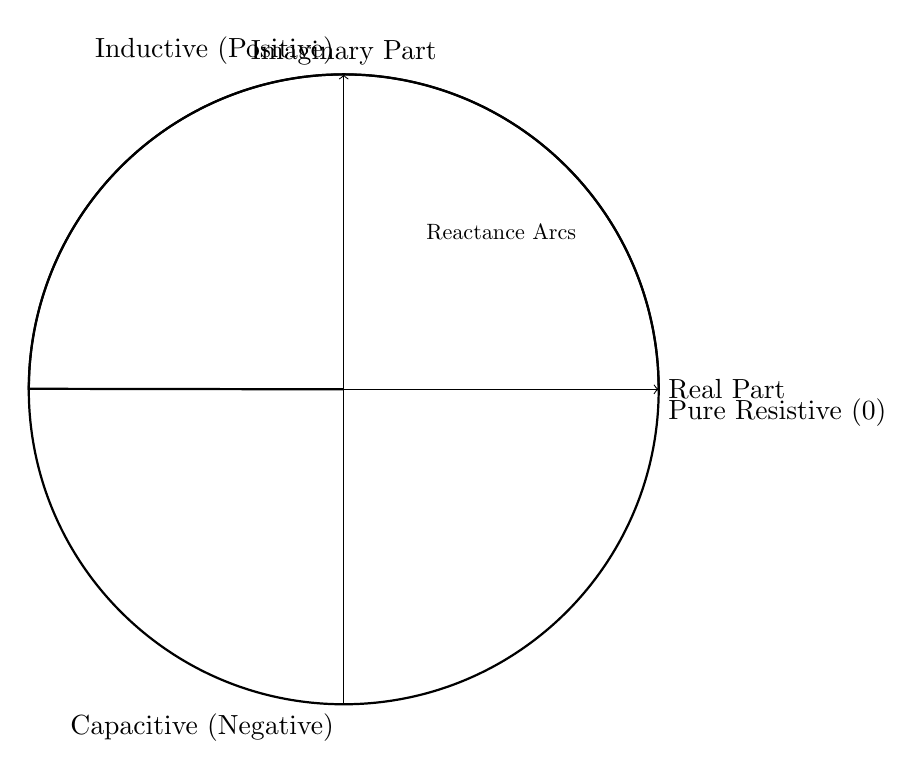
\begin{tikzpicture}
    \draw[->] (-4,0) -- (4,0) node[right] {Real Part};
    \draw[->] (0,-4) -- (0,4) node[above] {Imaginary Part};
    
    % Draw the outer circle
    \draw[thick] (0,0) circle (4);
    
    % Marking points for reactance
    \node at (4,0) [below right] {Pure Resistive (0)};
    \node at (0,4) [above left] {Inductive (Positive)};
    \node at (0,-4) [below left] {Capacitive (Negative)};
    
    % Reactance arcs
    \draw[domain=0:3.14/2,smooth,variable=\x,thick] plot ({4*cos(\x r)},{4*sin(\x r)});
    \draw[domain=3.14/2:3.14,smooth,variable=\x,thick] plot ({4*cos(\x r)},{4*sin(\x r)}) -- (0,0);
    
    % Labeling
    \node[scale=0.8] at (2,2) {Reactance Arcs};
\end{tikzpicture}
